\documentclass[t]{sdqbeamer}
%\documentclass[c]{sdqbeamer}

\usepackage{listings}
\usepackage{graphicx}
\usepackage{tabularx}
\usepackage{tikzsymbols}

\hypersetup{
	colorlinks=true,
	urlcolor=kit-orange
}

% set sdqbeamer options
\titleimage{blender-render}
\groupname{Algorithm Engineering}
\grouplogo{ae}
\selectlanguage{english}

% define title etc.pp.
\title[SAT Solving]{Practical SAT Solving}
\subtitle{Lecture 2}
\author{\underline{Markus Iser}, Dominik Schreiber, Tom\'a\v{s} Balyo}
\date{April 22, 2024}

% Existing KIT colors: kit-green, kit-blue, kit-red, kit-gray, kit-orange, kit-lightgreen, kit-brown, kit-purple, kit-cyan
% configure appearance
\setbeamercolor{block title}{bg=kit-blue}
\setbeamercolor{block body}{bg=kit-blue!10}
\setbeamercolor{block title example}{bg=kit-orange}
\setbeamercolor{block body example}{bg=kit-orange!10}
\setbeamertemplate{itemize item}{\color{kit-gray}\textbullet}
\setbeamertemplate{itemize subitem}{\color{kit-gray}\textbullet}
\setbeamercolor{item projected}{bg=kit-gray, fg=kit-gray}
\renewcommand{\insertnavigation}[1]{} % remove navigation bar

% define commands
\definecolor{myblue}{HTML}{0D3B66}
\definecolor{myred}{HTML}{6E0E0A}
\definecolor{mypink}{HTML}{F7B2B7}

\newcommand{\vars}[1]{\textsf{vars} (#1)}
\newcommand{\lits}[1]{\textsf{lits} (#1)}
\newcommand{\clss}[1]{\textsf{clss} (#1)}

\newcommand{\highl}[1]{\textcolor{myblue}{#1}}
\newcommand{\highlo}[1]{\textcolor{myred}{#1}}
\newcommand{\highlow}[1]{\textcolor{mypink}{#1}}

% Extra column types for tabularx
\newcolumntype{C}{>{\centering\arraybackslash}X}
\newcolumntype{L}{>{\raggedright\arraybackslash}X}
\newcolumntype{R}{>{\raggedleft\arraybackslash}X}

\newcommand{\setcolsep}[1]{\setlength{\tabcolsep}{#1}}
\newcommand{\setrowsep}[1]{\renewcommand{\arraystretch}{#1}}

% Definitions for the Tseitin transformation
\newcommand{\true}{\ensuremath{\mathit{True}}}
\newcommand{\false}{\ensuremath{\mathit{False}}}
\newcommand{\allvars}{\ensuremath{\mathcal{V}}}
\newcommand{\tseitin}[1]{\ensuremath{\mathcal{T}(#1)}}
\newcommand{\tseitinRec}[2]{\ensuremath{\mathcal{T}^{#2}(#1)}}
\newcommand{\tseitinSym}[1]{\ensuremath{\mathcal{T}_\mathsf{lit}(#1)}}
\newcommand{\tseitinDef}[2]{\ensuremath{\mathcal{T}_\mathsf{def}^{#2}(#1)}}
\newcommand{\hcancel}[2][black]{\setbox0=\hbox{$#2$}\rlap{\raisebox{.45\ht0}{\textcolor{#1}{\rule{\wd0}{1pt}}}}#2} 
\newcommand{\sateq}{\mathrel{\overset{\makebox[0pt]{\mbox{\normalfont\tiny\sffamily SAT}}}{=}}}

\newcommand{\enc}{\ensuremath{\mathcal{E}}} % encoding

% exercise commands
\newcommand{\exhead}[3]{
\hrule~\\[1ex]\noindent
{\bf Practical SAT Solving} (ST 2024) \hfill \fbox{Assignment #1} \\[1ex]
Markus Iser, Dominik Schreiber, Tom\'a\v{s} Balyo\\[1ex]
Algorithm Engineering (KIT) \hfill #2 -- #3\\
\hrule
\thispagestyle{empty}
}
\setlength{\itemsep}{1em}

\begin{document}

\begin{frame}
	\thispagestyle{empty}
	\titlepage
\end{frame}

\begin{frame}{Overview}
	\begin{block}{Recap. Lecture 1}
		\begin{itemize}\setlength{\itemsep}{1em}
			\item Satisfiability: Propositional Logic, CNF Formulas, NP-completeness, Applications
			\item Examples: Pythagorean Triples, Arithmetic Progressions, k-Colorability
			\item Incremental SAT: IPASIR, Sample Code
		\end{itemize}
	\end{block}
	\begin{block}{Today's Topics}
		\begin{itemize}\setlength{\itemsep}{1em}
			\item Tractable Subclasses
			\item Constraint Encodings
			\item Encoding Techniques
		\end{itemize}
	\end{block}
\end{frame}

\begin{frame}{Tractable Subclasses}
\pause
\begin{block}{Tractable Subclasses \href{https://doi.org/10.1145/800133.804350}{(cf.~Schaefer, 1978)}}
	\begin{itemize}\setlength{\itemsep}{1em}
		\item \textbf{2-SAT}\\Exactly two literals per clause
		\item \textbf{HORN-SAT}\\At most one positive literal per clause
		\item \textbf{Inverted HORN-SAT}\\At most one negative literal per clause
		\item \textbf{Positive / Negative}\\Literals occur only pure (either positive or negative)
		\item \textbf{XOR-SAT}\\No clauses, only XOR constraints
	\end{itemize}
\end{block}
\end{frame}

\begin{frame}{2-SAT}{aka.~Binary or Quadratic SAT}
Each clause has exactly two literals.
\begin{example}[2-SAT Formulas]
\vspace*{-3ex}
\begin{flalign*}
	F_5 &= \{ \{ x_1, x_2 \}, \{ \overline{x_1}, x_2 \}, \{ x_1, \overline{x_2} \}, \{ \overline{x_1}, \overline{x_2} \} \} &\\
	F_7 &= \{ \{ \overline{x_1}, x_2 \}, \{ \overline{x_2}, x_3 \}, \{ \overline{x_3}, x_1 \}, \{ x_2, x_4 \}, \{ x_3, x_4 \}, \{ x_1, x_3 \} \} &
\end{flalign*}
\end{example}
\pause
\begin{block}{Linear Time Algorithm for 2-SAT \href{https://doi.org/10.1016/0020-0190(79)90002-4}{(cf.~Aspvall et al., 1979)}}
	\begin{itemize}\setlength{\itemsep}{1em}
		\item \highl{Construct} Implication Graph:\\[1ex]
			  Directed graph with a vertex for each literal and two edges \highlo{$\overline l_1 \rightarrow l_2$} and \highlo{$\overline l_2 \rightarrow l_1$} for each clause $\{ l_1, l_2 \}$
		\item \highl{Find} Strongly Connected Components (SCC)\\[1ex]
			  \highlo{SCC:} There is a path from every vertex to every other vertex
		\item \highl{Check} for Complementary Literals in the same SCC
	\end{itemize}
\end{block}
\end{frame}

% \begin{frame}{How to solve 2-SAT?}
% \begin{block}{Saturation Algorithm}
% The resolution saturation algorithm is \highl{polynomial} for 2-SAT.
% \end{block}
% \textbf{Proof}
% \begin{itemize}
% 	\item Only 2-literal resolvents are possible
% 	\item There are only $\mathcal{O}(n^2)$ 2-literal clauses on $n$ variables
% \end{itemize}
% \textbf{Complexity}
% \begin{itemize}
% 	\item Both time and space $\mathcal{O}(n^2)$
% 	\item There exists a \highl{linear algorithm}! \cite{aspvall1979linear} \\($\mathcal{O}(n+m)$, where
% 	$m$ is the number of clauses)
% \end{itemize}
% \end{frame}

\begin{frame}{Implication Graph}
	
\begin{example}[Implication Graph]
	\centering
	\vspace*{1ex}
	\begin{columns}[T]
	\begin{column}{0.6\textwidth}
		$F_7 = \{ \{ \overline{x_1}, x_2 \}, \{ \overline{x_2}, x_3 \}, \{ \overline{x_3}, x_1 \}, \{ x_2, x_4 \}, \{ x_3, x_4 \}, \{ x_1, x_3 \} \}$\\[1ex]
		\only<2>{
			\begin{itemize}\setlength{\itemsep}{1em}
				\item Find \highl{Strongly Connected Components} (SCC)
				\item \highl{Tarjan's algorithm} finds SCCs in $\mathcal{O}(|V|+|E|)$
				\item \highlo{Complexity:} $\mathcal{O}(n+m)$, where $m$ is the number of clauses
			\end{itemize}
		}
		\only<3->{
			\begin{itemize}\setlength{\itemsep}{1em}
				\item If an SCC contains both $x$ and $\overline{x}$, the formula is \highlo{UNSAT}
				\begin{itemize}\setlength{\itemsep}{1ex}
					\only<3>{\item Why?}
					\item<4-> $x$ implies its own negation!
					\item<4-> Literals in an SCC must be either all true or all false
				\end{itemize}
				\item<4-> What about \highlo{SAT}? How to get a solution?
				\begin{itemize}\setlength{\itemsep}{1ex}
					\item<5-> Contract each SCC into one vertex
					\item<5-> In reverse topological order, set unassigned literals to \texttt{true}.
					% \item Example: $x_1 = x_2 = x_3 = \texttt{true}$, $x_4 = \texttt{true}$, the rest is already assigned.
				\end{itemize}
			\end{itemize}
		}
	\end{column}%
	\begin{column}{0.3\textwidth}
		\only<1>{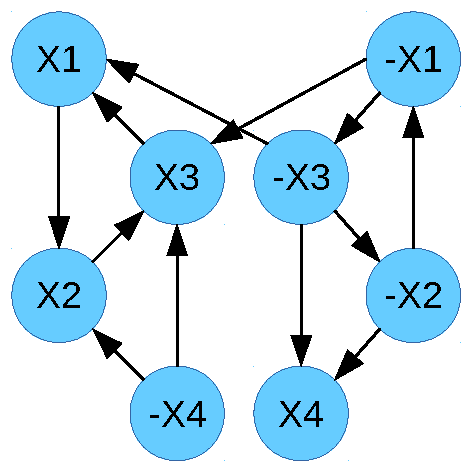
\includegraphics[width=.9\textwidth]{figures/l02/impgraph.pdf}}
		\only<2-4>{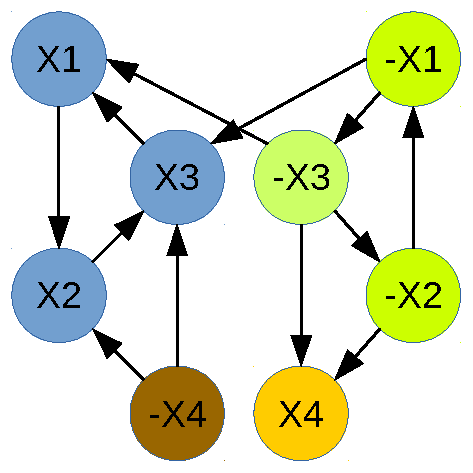
\includegraphics[width=.9\textwidth]{figures/l02/impgraph-comp.pdf}}
		\only<5>{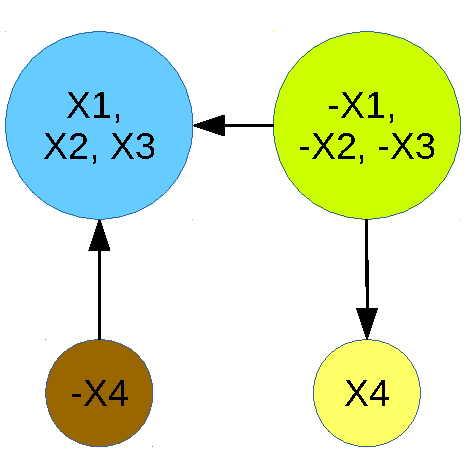
\includegraphics[width=.9\textwidth]{figures/l02/impgraph-cond.pdf}}
	\end{column}
	\end{columns}
\end{example}
\end{frame}


\begin{frame}{HornSAT}
	Each clause contains at most one positive literal.
	\begin{example}[Horn Formula]
		Each clause can be written as an implication with \highl{positive literals only and a single consequent}:
		\vspace*{-1ex}
		\begin{flalign*}
			F_6 &= \bigl\{ \{ \overline{x_1}, x_2 \}, \{ \overline{x_1}, \overline {x_2}, x_3 \}, \{ x_1 \} \bigr\} &\\
				&\equiv \bigl(x_1 \rightarrow x_2\bigr) \wedge \bigl((x_1 \wedge x_2) \rightarrow x_3\bigr) \wedge \bigl(\top \rightarrow x_1\bigr) &
		\end{flalign*}
	\end{example}
	\pause
	\begin{block}{Solving Horn Formulas}
		\begin{itemize}
			\item Propagate until fixpoint
			\item If $\top \rightarrow \bot$ then the formula is \highlo{UNSAT}. Otherwise it is \highl{SAT}.
			\item Construct a satisfying assignment by setting the remaining variables to \texttt{false}
		\end{itemize}
	\end{block}
\end{frame}

\begin{frame}{Hidden Horn}{aka. Renamable or Disguised Horn}
	A CNF formula is \highl{Hidden Horn} if it can be made \highl{Horn} by flipping the polarity of some of its variables.
	\begin{example}[Hidden Horn Formula]
		\vspace*{-3ex}
		\begin{flalign*}
			F_8 = &\{ \{ x_1, x_2, x_4 \}, \{ x_2, \overline{x_4} \}, \{ x_1 \} \} &\\
			\leadsto &\{ \{ \overline{x_1}, \overline{x_2}, x_4 \}, \{ \overline{x_2}, \overline{x_4} \}, \{ \overline{x_1} \} \} &
		\end{flalign*}
	\end{example}
	\highl{How to recognize} a Hidden Horn formula? \highlo{And how to hard is it?}
	\pause
	\begin{block}{Recognizing Hidden Horn Formula $F$}
		Construct 2-SAT formula $R_F$ that contains the clause $\{l_1, l_2\}$ iff there is a clause $C \in F$ such that $\{l_1, l_2\} \subseteq C$.\\[1ex]
		\begin{itemize}\setlength{\itemsep}{1em}
			\item Example: $R_{F_8} = \{ \{ x_1, x_2 \}, \{ x_1, x_4 \}, \{ x_2, x_4 \}, \{ x_2, \overline{x_4} \} \}$
			\item If the 2-SAT formula is satisfiable, then $F$ is Hidden Horn
			\item If $x_i = \texttt{true}$ in $\phi$, then $x_i$ needs to be renamed to $\overline x_i$
		\end{itemize}
	\end{block}
\end{frame}

\begin{frame}{Mixed Horn}
	A CNF formula is \highl{Mixed Horn} if it contains only binary and Horn clauses.
	\begin{example}[Mixed Horn Formula]
		\vspace*{-3ex}
		\begin{flalign*}
			F_9 = &\{ \{ \overline{x_1}, \overline{x_7}, x_3 \}, \{ \overline{x_2}, \overline{x_4} \}, \{ x_1, x_5 \}, \{ x_3 \} \} &
		\end{flalign*}
	\end{example}
	\highl{How to solve} a Mixed Horn formula? \highlo{And how to hard is it?}
	\pause
	\begin{block}{Mixed Horn is NP-complete}
		\textbf{Proof}: \highl{Reduce SAT} to Mixed Horn SAT\\[1ex]
		For each non-Horn non-binary clause $C=\{l_1, l_2, l_3, \dots\}$, 
		\begin{itemize}\setlength{\itemsep}{1ex}
			\item for each but one positive $l_i$ $\in C$ introduce a new variable $l'_i$ and replace $l_i$ in $C$ by $\overline{l'_i}$
			\item add clauses $\{ l'_i, l_i \}, \{ \overline{l'_i}, \overline{l_i} \}$ to establish $l_i = \overline{l'_i}$
		\end{itemize}
	\end{block}
\end{frame}

\begin{frame}{Next up: CNF Encodings}
	\begin{block}{Elementary Encodings}
		\begin{itemize}\setlength{\itemsep}{1ex}
			\item Tseitin Transformation
			\item Cardinality Constraints
			\item Finite Domain Encodings
		\end{itemize}
	\end{block}
	\begin{block}{Properties of Encodings}
		\begin{itemize}\setlength{\itemsep}{1ex}
			\item Size: Number of Variables and Clauses
			\item Propagation consistency: Can the encoding ensure consistency through propagation?
		\end{itemize}
	\end{block}
\end{frame}


\begin{frame}{Encoding Circuits}
	Given a propositional formula $F$ with operations $\wedge$, $\vee$, and $\lnot$, how can it be encoded in CNF?
	\begin{example}[CNF Conversion]
		\vspace*{-3ex}
		\begin{align*}
			F =&\, \lnot((\lnot x \lor y) \land (\lnot z \land \lnot (x \land \lnot w))) \tag{Given Formula} \\[1ex]
			\visible<2->{
				=&\, (x \land \lnot y) \lor z \lor (x \land \lnot w) \tag{Negation Normal Form} \\[1ex]
			}
			\visible<3->{
				=&\, (x \lor z) \land (x \lor z \lor \lnot w) \land (\lnot y \lor z \lor x) \land (\lnot y \lor z \lor \lnot w) \tag{Conjunctive Normal Form} \\
			}
		\end{align*}
	\end{example}
	\begin{block}{Naive / Direct Conversion}
		\begin{itemize}\setlength{\itemsep}{1ex}
			\item<2-> Convert to Negation Normal Form (NNF)
			\item<3-> Apply distributive law to get CNF
			\item<3-> Problem: Applying the distributive law may result in an exponential blow-up.
		\end{itemize}
	\end{block}
\end{frame}

\begin{frame}{Tseitin Encoding}
Idea: Introduce new variables for subformulas.
\begin{example}[Tseitin Conversion]
	\begin{columns}
	\begin{column}{0.6\textwidth}
		\vspace*{-3ex}
		\begin{align*}
			F =&\, (x \land \lnot y) \lor z \lor (x \land \lnot w) \tag{Negation Normal Form} \\[1ex]
			  \sateq &\, (c \leftrightarrow x \land \lnot w) \land \dots \land (f \leftrightarrow a \lor b) \land f \tag{Tseitin Encoding}
		\end{align*}
		\begin{itemize}\setlength{\itemsep}{1ex}
			\item Define new variables: $a \leftrightarrow x \land \overline{y}, \quad f \leftrightarrow a \lor b, \quad \dots$
			\item Encode definitions in CNF:
				$(\overline{f} \lor a \lor b) \land (f \lor \overline{a}) \land (f \lor \overline{b}) \land \dots$
			\item One additional clause $(f)$ to assert that $F$ must be true
		\end{itemize}
	\end{column}
	\begin{column}{0.4\textwidth}
	\begin{center}
		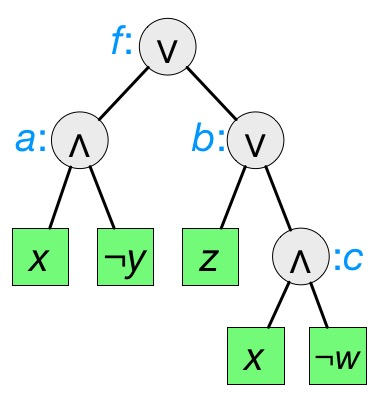
\includegraphics[height=0.6\textwidth]{figures/l02/formula-graph-2.jpg}
	\end{center}
	\end{column}
	\end{columns}
\end{example}
\end{frame}

\begin{frame}{Tseitin Encoding}
The Tseitin-Encoding $\tseitin{F}$ of a propositional formula $F$ over connectives $\{ \land, \lor, \lnot \}$ is specified as follows.
\begin{block}{Definition of Tseiting Encoding}
	\vspace*{-3ex}
	\begin{align*}
	\tseitin{F} &= d_F \wedge \tseitinRec{F}{*} \tag{Root Formula}\\[1ex]
	\tseitinRec{F}{*} &= \begin{cases}
			\tseitinDef{F}{} \wedge \tseitinRec{G}{*} \wedge \tseitinRec{H}{*},
				& \text{if } F = G \circ H \text{ and } \circ \in \{\wedge, \vee\}\\
			\tseitinDef{F}{} \wedge \tseitinRec{G}{*}, & \text{if } F = \neg G\\
			\true, & \text{if } F \in \allvars
		\end{cases} \tag{Recursion}\\[1ex]
	\tseitinDef{F}{} &= \begin{cases}
			(\overline{d_F} \vee d_G) \wedge (\overline{d_F} \vee d_H) \land
				(d_F \lor \overline{d_G} \lor \overline{d_H}), & \text{if } F = G \wedge H\\
			(\overline{d_F} \vee d_G \vee d_H) \lor (d_F \vee \overline{d_G}) \wedge 
				(d_F \vee \overline{d_H}) , & \text{if } F = G \vee H\\
			(\overline{d_F} \lor \overline{d_G}) \land (d_F \lor d_G), & \text{if } F = \neg G \tag{Definitions}\\
			\end{cases}
	\end{align*}
\end{block}
\highlo{$\tseitin{F}$} introduces a new variable $d_S$ for each subformula $S$ of $F$ and \highlo{is satisfiable iff $F$ is satisfiable}.
\end{frame}

\begin{frame}{Tseitin Encoding}
	\begin{example}[Tseitin Encoding]
		\vspace*{-3ex}
		\begin{align*}
			F =&\, \underbrace{\overbrace{(x \land \lnot y)}^{a,\;S_a} \lor
			\underbrace{(z \lor \overbrace{(x \land \lnot w)}^{c,\;S_c})}_{b,\;S_b}}_f \tag{Encoding / Auxiliary Variables}\\[1ex]
			\sateq & \tseitinDef{S_c}{} \land \tseitinDef{S_b}{} \land \tseitinDef{S_a}{} \land \tseitinDef{F}{} \land f\\[1ex]
			\sateq & \dots \land \underbrace{(f \lor \overline{a}) \land (f \lor \overline{b}) \land (\overline{f} \lor a \lor b)}_{\tseitinDef{F}{}} \,\land\, f \tag{Tseitin Encoding} \\[1ex]
			\sateq &\, (c \leftrightarrow x \land \lnot w) \land \dots \land (f \leftrightarrow a \lor b) \land f
		\end{align*}
	\end{example}
	\highlo{Simplification:} treat negative literals like variables in $\tseitin{F}$
\end{frame}

\begin{frame}{Tseitin Encoding: Plaisted-Greenbaum Optimization}
	\begin{example}[Plaisted-Greenbaum Optimization]
		\vspace*{-3ex}
		\begin{align*}
		\only<1>{
			\tseitin{F}
			&= f \land (f \leftrightarrow a \lor b) \land (a \leftrightarrow x \land \lnot y) \land (b \leftrightarrow z \lor c) \land (c \leftrightarrow x \land \lnot w) \\[1ex]
			&= f \land (\overline{f} \lor a \lor b) \land (f \lor \overline{a}) \land (f \lor \overline{b}) \\
			& \quad\;\;\; \land (\overline{a} \lor x) \land (\overline{a} \lor \overline{y}) \land (a \lor \overline{x} \lor y) \\
			& \quad\;\;\; \land (\overline{b} \lor z \lor c) \land (b \lor \overline{z}) \land (b \lor \overline{c}) \\
			& \quad\;\;\; \land (\overline{c} \lor x) \land (\overline{c} \lor \overline{w}) \land (c \lor \overline{x} \lor w)
		}
		\only<2>{
			\mathcal{T}^{PG}(F)
			&= f \land (f \highlo{\boldsymbol{\rightarrow}} a \lor b) \land (a \highlo{\boldsymbol{\rightarrow}} x \land \lnot y) \land (b \highlo{\boldsymbol{\rightarrow}} z \lor c) \land (c \highlo{\boldsymbol{\rightarrow}} x \land \lnot w) \\[1ex]
			&= \hcancel[myred]{f} \land (\overline{\hcancel[myred]{f}} \lor a \lor b) \land \hcancel[myred]{(f \lor \overline{a})} \land
				 \hcancel[myred]{(f \lor \overline{b})} \\
			& \quad\;\;\; \land (\overline{a} \lor x) \land (\overline{a} \lor \overline{y}) \land
				 \hcancel[myred]{(a \lor \overline{x} \lor y)} \\
			& \quad\;\;\; \land (\overline{b} \lor z \lor c) \land \hcancel[myred]{(b \lor \overline{z})}
				 \land \hcancel[myred]{(b \lor \overline{c})} \\
			& \quad\;\;\; \land (\overline{c} \lor x) \land (\overline{c} \lor \overline{w}) \land
				\hcancel[myred]{(c \lor \overline{x} \lor w)} \\
			&\sateq (a \lor b) \land (\overline{a} \lor x) \land (\overline{a} \lor \overline{y}) \land
				(\overline{b} \lor z \lor c) \land (\overline{c} \lor x) \land (\overline{c} \lor \overline{w})
		}
		\end{align*}
	\end{example}
	\highlo{Relaxed Transformation: } Exploit \emph{Don't Cares} in monotonic functions\\[1ex]
	\highlo{Model Duplication: } Unconstrained encoding variables introduce additional models \\[1ex]
	\highlo{Semantic Coupling: } $\tseitin{F} \models \mathcal{T}^{PG}(F) \models F$
\end{frame}

\begin{frame}{Tseitin Encoding: Plaisted-Greenbaum Optimization}
\begin{block}{Definition of \href{http://dx.doi.org/10.1016/S0747-7171(86)80028-1}{Plaisted Greenbaum Encoding}}
	\vspace*{-3ex}
	\begin{align*}
	\tseitin{F} &= d_F \wedge \tseitinRec{F}{1}\\
	\tseitinRec{F}{p} &= \begin{cases}
			\tseitinDef{F}{p} \wedge \tseitinRec{G}{p} \wedge \tseitinRec{H}{p},
				& \text{if } F = G \circ H \text{ and } \circ \in \{\wedge, \vee\}\\
			\tseitinDef{F}{p} \wedge \tseitinRec{G}{p \oplus 1}, & \text{if } F = \neg G\\
			\true, & \text{if } F \in \allvars
		\end{cases}\\
	\tseitinDef{F}{1} &= \begin{cases}
			(\overline{d_F} \vee d_G) \wedge (\overline{d_F} \vee d_H), & \text{if } F = G \wedge H\\
			(\overline{d_F} \vee d_G \vee d_H), & \text{if } F = G \vee H\\
			(\overline{d_F} \vee \overline{d_G}), & \text{if } F = \neg G\\
			\end{cases}\\
	\tseitinDef{F}{0} &= \begin{cases}
			(d_F \vee \overline{d_G} \vee \overline{d_H}), & \text{if } F = G \wedge H\\
			(d_F \vee \overline{d_G}) \wedge (d_F \vee \overline{d_H}), & \text{if } F = G \vee H\\ 
			(d_F \vee d_G), & \text{if } F = \neg G
		\end{cases}
	\end{align*}
\end{block}
\end{frame}


\begin{frame}{Recap}

\begin{block}{Elementary Encodings}
	\begin{itemize}\setlength{\itemsep}{1em}
		\item Tseitin Transformation
		\begin{itemize}\setlength{\itemsep}{1ex}
			\item Tseitin encoding allows to carry over structure to CNF
			\item Formula size linear in the number of subformulas (of bounded arity)
		\end{itemize}
		\item Cardinality Constraints
		\item Finite Domain Encodings
	\end{itemize}
\end{block}
\pause
\begin{block}{Next Up}
	Cardinality Constraints
\end{block}

\end{frame}


\begin{frame}{At-Most-One Constraints}{Notation: $\operatorname{AtMostOne}(x_1, \dots, x_n)$ or $\leq\!1\,(x_1, \dots, x_n)$ or $\sum_i^n x_i \leq 1$}
	Not more than one literal from $x_1, \dots, x_n$ is set to True.

	\begin{block}{Naive / Pairwise Encoding}
		\begin{tabularx}{\linewidth}{LR}
		$\enc\bigl[\leq\!1\,(x_1, \dots, x_n)\bigr] = \bigl\{ \{\overline{x_i}, \overline{x_j} \} \mid 1 \leq i < j \leq n \bigr\}$ 
		& Size: ${n \choose 2} = \frac{n \cdot (n-1)}{2}$ clauses
		\end{tabularx}
	\end{block}
	\begin{block}{Size Complexity}
		\centering\setcolsep{10pt}\setrowsep{1.5}
		\begin{tabularx}{\linewidth}{XlXl}
			\bf Encoding & \bf Clauses & \bf Enc. Variables & \bf Consistency \\
			\hline
			Pairwise Encoding & $\mathcal{O}(n^2)$ & 0 & direct \\
			Tree Encoding & $\mathcal{O}(n \log n)$ & $\log n$ & propagate \\
			Ladder Encoding & $\mathcal{O}(n)$ & $n$ & propagate
		\end{tabularx}
	\end{block}
\end{frame}

\begin{frame}{Cardinality Constraints}{Notation: $\leq\!k\,(x_1, \dots, x_n)$ or $\sum_i^n x_i \leq k$}
	Not more than $k$ literals from $x_1, \dots, x_n$ are set to True.
	\begin{block}{Naive Encoding}
		\begin{tabularx}{\linewidth}{lR}
			$\enc\bigl[\leq\!k\,(x_1, \dots, x_n)\bigr] = \bigl\{ \{\overline{x_{i_1}}, \dots, \overline{x_{i_{k+1}}} \} \mid 1 \leq i_1 < \dots < i_{k+1} \leq n \bigr\}$ 
			& Size: ${n \choose k+1}$ clauses\footnote{$\approx 2^n/\sqrt{n}$ by Stirling's Approx. for the worst case $k = \lceil n/2 \rceil$}
		\end{tabularx}
	\end{block}
	\begin{block}{Size Complexity}
		\centering\setcolsep{10pt}\setrowsep{1.5}
		\begin{tabularx}{\linewidth}{XlXl}
			\bf Encoding & \bf Clauses & \bf Enc. Variables & \bf Consistency \\
			\hline
			Naive Encoding & ${n \choose k+1}$ & 0 & direct\\
			Sequential Counter Encoding & $\mathcal{O}(n \cdot k)$ & $\mathcal{O}(n \cdot k)$ & propagate \\
			Parallel Counter Encoding & $\mathcal{O}(n)$ & $\mathcal{O}(n)$ & search
		\end{tabularx}
	\end{block}
\end{frame}

\begin{frame}{Cardinality Constraints: Sequential Counter Encoding}{Idea: encode count-and-compare hardware circuit (cf.~\href{https://doi.org/10.1007/11564751\_73}{Sinz, 2005})}
	\begin{tikzpicture}[remember picture, overlay]
		\node[xshift=70pt,yshift=30pt] at (current page.center) {
			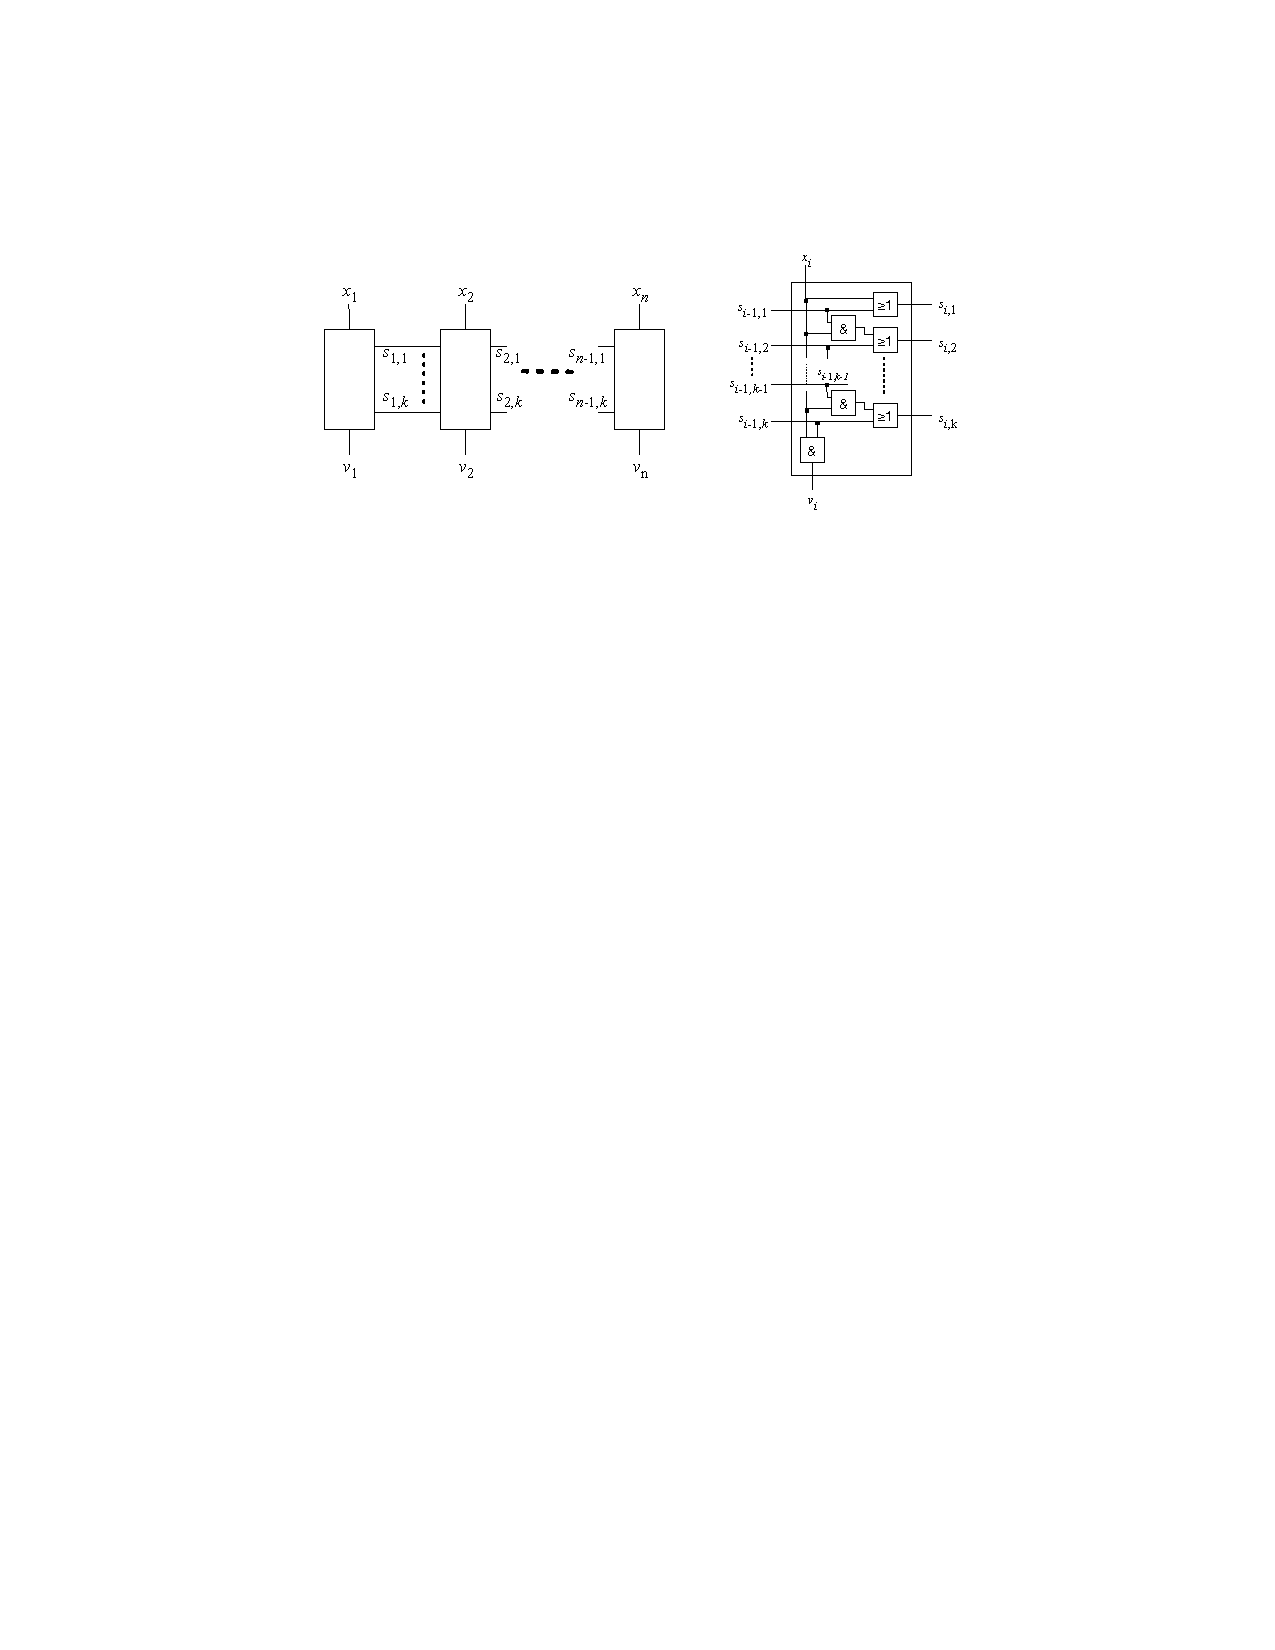
\includegraphics[height=0.42\textheight]{figures/l02/seq-counter-1.pdf}
		};
		\node[xshift=-90pt,yshift=-50pt] at (current page.center) {
			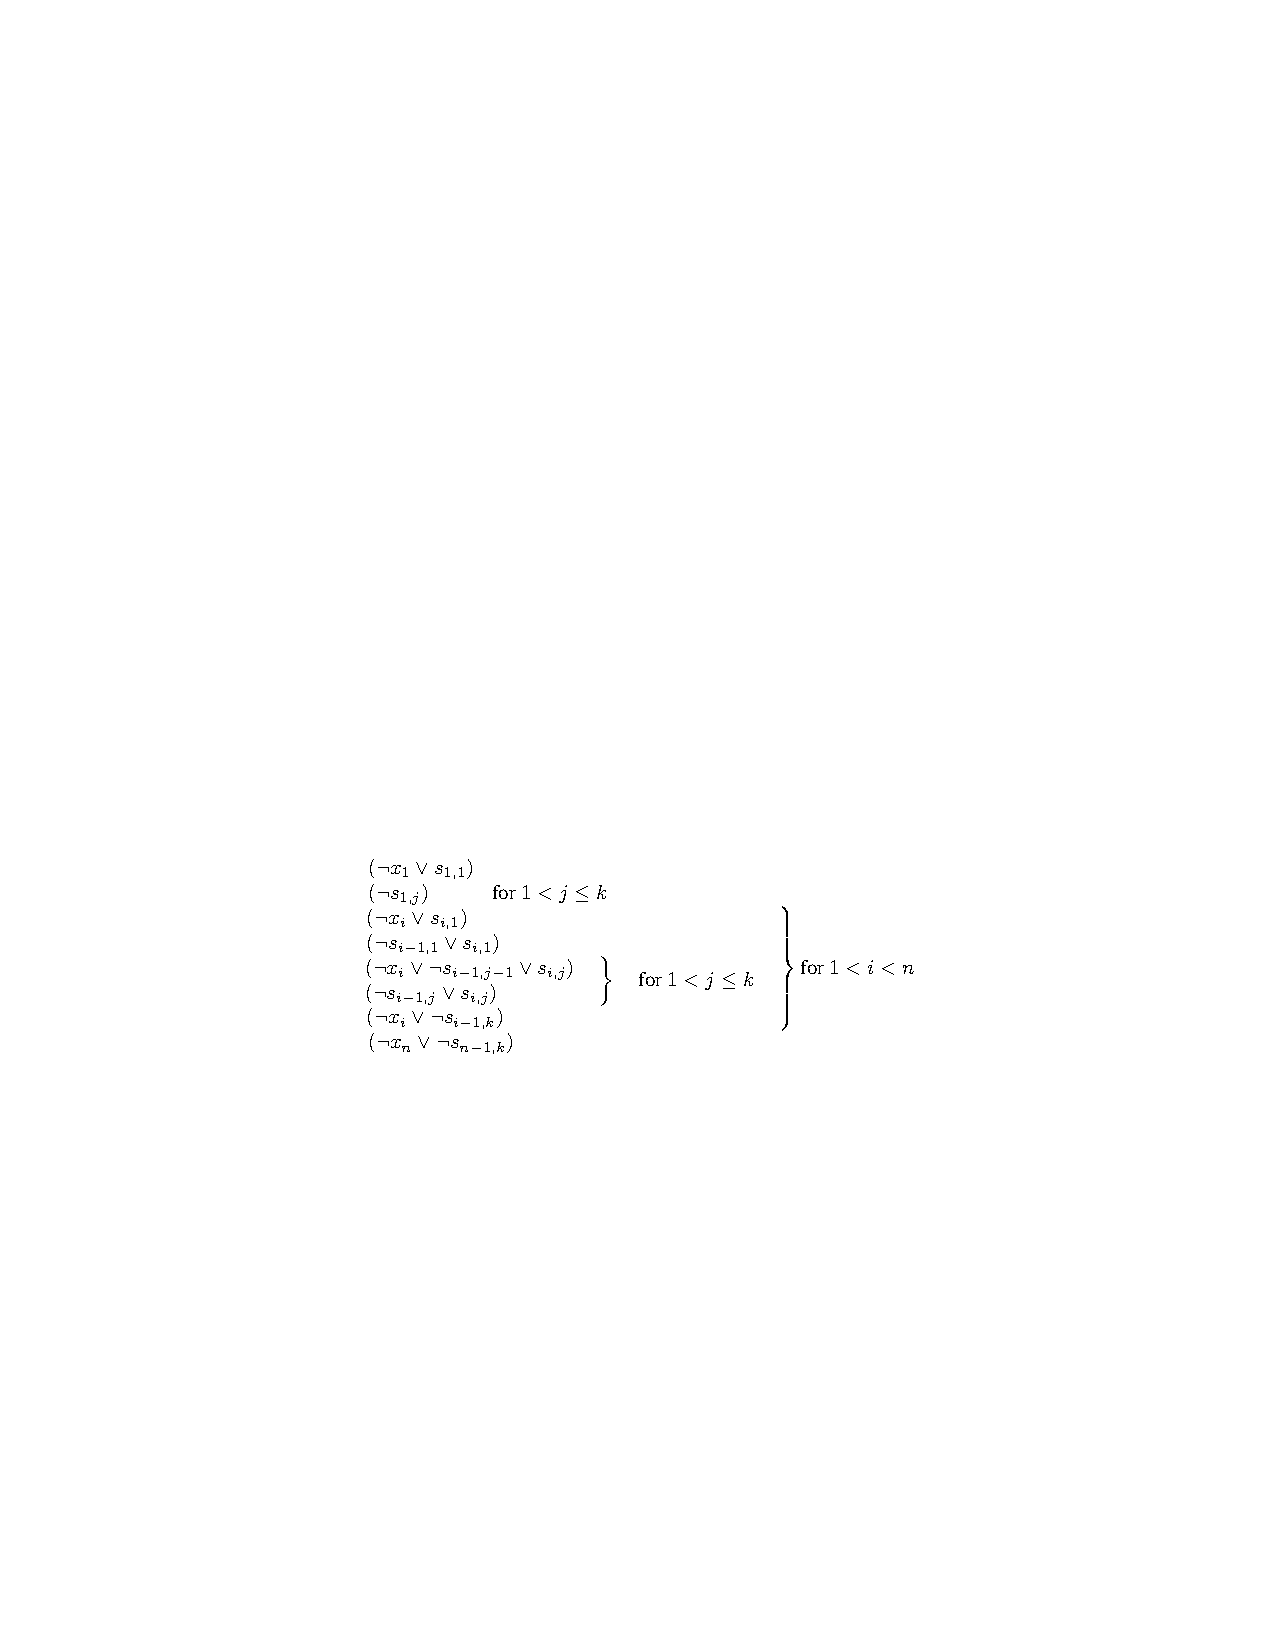
\includegraphics[height=0.4\textheight]{figures/l02/seq-counter-2.pdf}
		};
	\end{tikzpicture}
\end{frame}

\begin{frame}{Recap}

	\begin{block}{Elementary Encodings}
		\begin{itemize}\setlength{\itemsep}{1em}
			\item Tseitin Transformation
			\begin{itemize}\setlength{\itemsep}{1ex}
				\item Tseitin encoding allows to carry over structure to CNF
				\item Formula size linear in the number of subformulas (of bounded arity)
			\end{itemize}
			\item Cardinality Constraints
			\begin{itemize}\setlength{\itemsep}{1ex}
				\item Size of encoding vs. Complexity of consistency
				\item Choice of encoding matters
			\end{itemize}
			\item Finite Domain Encodings
		\end{itemize}
	\end{block}
	\pause
	\begin{block}{Next Up}
		Finite Domain Encodings
	\end{block}
	
\end{frame}

\begin{frame}{Finite-Domain Variables}
	Common in combinatorial problems: finite domain variables, e.g.: $x \in \{ v_1, \dots, v_n \}$\\
	Relationships between them expressed as equality-formulas, e.g.: $x = v_3 \Rightarrow y \neq v_2$.
	\begin{block}{Direct encoding / ``one-hot-encoding''}
		\begin{itemize}
		\item Boolean variables $x_v$: ``x takes value v''
		\item Must encode that each variable takes exactly one value from its domain
			(using at-least-one/at-most-one constraints)
		\item Encoding of variables' constraints simple
		\end{itemize}
	\end{block}
\end{frame}
\begin{frame}{Finite-Domain Variables}
	Common in combinatorial problems: finite domain variables, e.g.: $x \in \{ v_1, \dots, v_n \}$\\
	Relationships between them expressed as equality-formulas, e.g.: $x = v_3 \Rightarrow y \neq v_2$.
	\begin{block}{Log-encoding / binary encoding}
		\begin{itemize}
		\item Boolean variables $b^x_i$ for $0 \leq i < \lceil \log_2{n} \rceil$
		\item Each value gets assigned a binary number, e.g. $v_1 \rightarrow 00, v_2 \rightarrow 01, v_3 \rightarrow 10$
		\item Inadmissible values must be excluded, e.g.: \\
			$x \in \{ v_1, v_2, v_3 \}$ requires $(\overline{b^x_0} \lor \overline{b^x_1})$
		\item Encoding of constraints can become complicated
		\end{itemize}
	\end{block}
\end{frame}

\begin{frame}{Recap}

	\begin{block}{Elementary Encodings}
		\begin{itemize}\setlength{\itemsep}{1em}
			\item Tseitin Transformation
			\begin{itemize}\setlength{\itemsep}{1ex}
				\item Tseitin encoding allows to carry over structure to CNF
				\item Formula size linear in the number of subformulas (of bounded arity)
			\end{itemize}
			\item Cardinality Constraints
			\begin{itemize}\setlength{\itemsep}{1ex}
				\item Size of encoding vs. Complexity of consistency
				\item Choice of encoding matters
			\end{itemize}
			\item Finite Domain Encodings
			\begin{itemize}\setlength{\itemsep}{1ex}
				\item One-hot encoding vs. Log encoding
				\item One-hot often simpler w.r.t. interaction between encodings
			\end{itemize}
		\end{itemize}
	\end{block}
	
\end{frame}

\end{document}
